% tGISguide.tex
% v3.2 released September 2006

\documentclass[printer]{tGIS2e}

\usepackage{url}
\usepackage{subfigure}

\def\Cplusplus{{\rm C\raise.5ex\hbox{\small ++}}}

\begin{document}
\markboth{Joana Sim\~{o}es, Chris Skelly and Jo\~{a}o Sim\~{o}es}{Iesim: simulating and understanding real world events in a game-like environment}

\title{Iesim: simulating and understanding real world events in a game-like environment}

%\author{Joana Sim\~{o}es$^{\ast}$$\dag$\thanks{$^\ast$Corresponding author. Email: j.simoes@ucl.ac.uk
\author{Joana Sim\~{o}es${\dag}$${\ddag}$${\bullet}$\thanks{$^\ast$Corresponding author. Email: j.simoes@ucl.ac.uk
\vspace{6pt}}, Chris Skelly${\bullet}$, Jo\~{a}o Sim\~{o}es${\star}$${\circ}$\\\vspace{6pt}  $\dag$ e-GEO, Faculdade de Ci\^{e}ncias Sociais e Humanas, UNL
Avenida de Berna, 26-C
1069-061 Lisboa,
Portugal.\\
$\ddag$ CASA,
 University College London,
 1 - 19 Torrington Place,
 London
 WC1E 7HB, UK.\\
$\bullet$ ieSim Org, London, UK.\\
$\star$ SIM, FCUL, Edif\'{i}cio C8, gab 8.5.12 1749-016 Lisboa, Portugal.\\
$\circ$  CERN, CH - 1211 Gen\'{e}ve 23, Swisse.\\
\vspace{6pt}\received{v1.0 released December
2009} }

\maketitle

\begin{abstract}
Iesim~\citep{iesim} is a software platform designed to simulate real-world community events in a friendly \textit{game-like} environment. It can be used for evaluating the effectiveness of interventions and predict and understand how events will unfold, and it can also be a valuable tool for training/education.\\
This papper describes an application using IesimLib library and environment, which implements an infectious disease model through which the user can simulate an hazard such as Flu or HIV. We will focus on some technical aspects of the software and User Interface (UI), but will also discuss the underlying model: and Agent Based Model (ABM); The use of Geographical Information Systems (GIS) concepts and algorithms was fundamental for generating and managing realistic spatial scenarios and it justified the development of an \textit{in-house} GIS library.
\end{abstract}
\bigskip

    \begin{keywords} Simulation Tool, Intervention Strategies, Education, cross-plattform, UI, GIS;\end{keywords}\bigskip

\section{Extended Abstract}\label{sec:extended}

\textit{OutbreakP2P} is a package for person-to-person diseases simulation, that demonstrates the potentialities of Iesim, for users and developers. It consists of an user interface (\textit{Intervene}) and a set of plugins that implement the different aspects of the model: community, hazard and intervention (\textit{ICom}, \textit{Ihaz} and \textit{IInt})\\

  \begin{figure}[!ht]%[htbp]
    \begin{center} 
	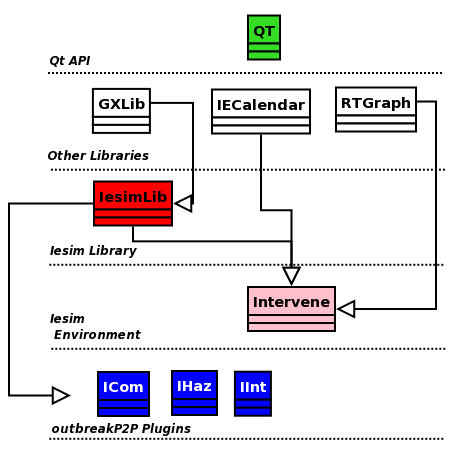
\includegraphics[width=0.6\textwidth]{pics/intervene2}%{pics/ib.png}\\
      \caption[Structure of Iesim Software;]{Structure of Iesim Software;}
      \label{1:01} % so that one can \ref it elsewhere	
    \end{center} 
  \end{figure}
Figure~\ref{1:01}, page~\pageref{1:01} shows the structure of the software: on a first level, Nokia's \textit{Qt}~\footnote{http://qt.nokia.com/products}
 provides a set of classes to develop the UI and other aspects (multithreading, etc); \textit{IesimLib} is the  library which puts together the core functionality split into small libraries (GIS, graphics, etc) and that is used to build both, the main application and the plugins.\\
The program was fully implemented in \Cplusplus and apart from \textit{Qt} it has no other dependencies, which means it is truly cross-plattform (see figure~\ref{1:02}, page~\pageref{1:02}).\\

\begin{figure}[!ht]
\centering
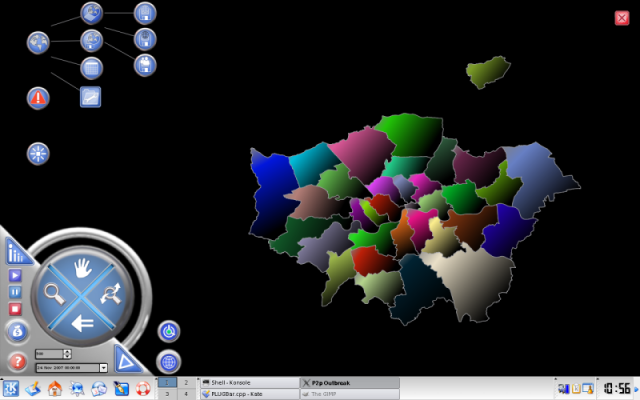
\includegraphics[height=0.3\textwidth]{pics/linuxScreen}
\subfigure[]{{}} 
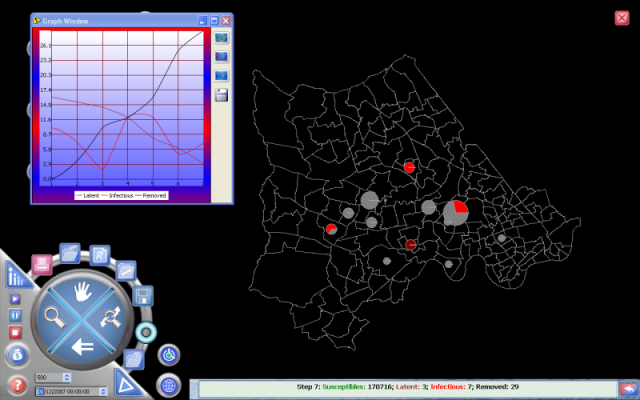
\includegraphics[height=0.3\textwidth]{pics/winScreen}
\subfigure[]{{}} 
\caption[Screenshots of OutbreakP2P, running in a) Linux and b) Windows desktop;]{Screenshots of OutbreakP2P, running in a) Linux and b) Windows desktop;}
\label{1:02} % so that one can \ref it elsewhere	
\end{figure}
One of the main concerns on the development of this product was to have an intuitive user interface (like in games), that does not require the user to go through complicated manuals for setting up a simulation. Another concern, was to be able to cope with the lack of data, so common when dealing with real case studies, by means of \textit{generating} information in an automatic or assisted way, just like it happens in games (\textit{e.g.}, \textit{Sim City}~\footnote{http://en.wikipedia.org/wiki/SimCity}). The idea was to have a model which will be as accurate as possible in the event of data availability, but that can  also serve as a tool for training or education in the event of no data, creating and exploring fictitious scenarios (see figure~\ref{1:03}, page~\pageref{1:03}).\\

  \begin{figure}[!ht]%[htbp]
   \begin{center} 
	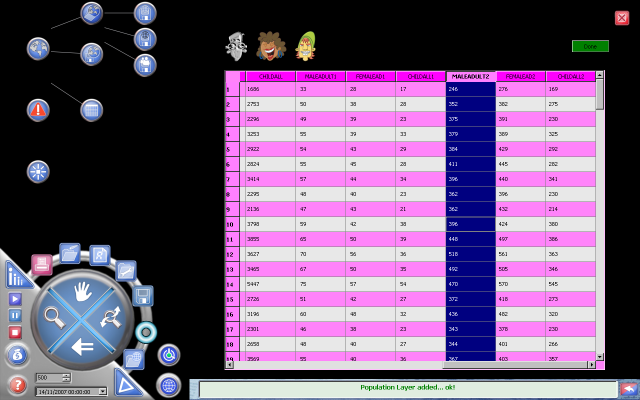
\includegraphics[width=0.8\textwidth]{pics/load_population}
      \caption[Loading population data, used to generate the communities;]{Loading population data, used to generate the communities;}
      \label{1:03} % so that one can \ref it elsewhere	
    \end{center} 
  \end{figure}

The model underneath OutbreakP2P is a spatially explicit agent based model (ABM) for the spreading of infectious diseases in human populations. Human-environment systems, are characterized by heterogeneity, nonlinear relationships, and hierarchical structures that give rise to difficulties in understanding system behavior in response to exogenous factors ~\citep{Li2005}. This kind of systems, that we define broadly as complex systems, are composed of many parts coupled together in a nonlinear fashion and tipically present self organization, a behavior in which order may arise from low level interactions without any supervision from higher-order structures~\citep{Nowak1996}. The bottom-up approach is the \textit{natural} way of studying these systems~\citep{Simoes2007}; however, the fact that there are a lot of random components has the consequence that the results cannot be reproduced like in deterministic models, and therefore each run of the model is often unique.\\
There are two assumptions that are crucial to the development of this model; one is that the spread of the disease relies strongly on social networks that are  nowhere near random, but present a certain structure: this led us to the development of a community model; the other was to relax the common assumptions of homogeneous mixing in an homogenous space and create a scenario with an irregular distribution of individuals in an irregular space; the strong spatial component of the model, which in itself brings a lot of complexity led to the development of a Geographic Information Systems (GIS) \textit{in-house} library.\\
One of the advantages of this kind of simulation tools is the ability to introduce and evaluate intervention strategies, such as vaccination~\citep{Simoes2007}; Like in the other input, this can be done by reading data, generating data with sub-models or simply and quickly clicking on the screen.\\
A realistic spatial simulation model can be the basis for simulating spatial intervention strategies and therefore be an important tool for planners and policy makers in any field. Learning the lesson from computer games, we also hope to have created a software that is easy to use by non-technical users, through a user-friendly user interface.\\

\bibliographystyle{tGIS}
\bibliography{tGISguide}


\end{document}

